% Emacs settings: -*-mode: latex; TeX-master: "manual.tex"; -*-

\chapter{Running \MCS}

This chapter describes the installation and usage of the McStas software.
The software should compile without problems on most Unix-like
systems with an ANSI-compliant C compiler. It has also been successfully
compiled on Windows and MacIntosh systems, but these platforms are
not actively supported. In case of problems, the McStas
mailing list~\cite{mcstas_webpage} or the authors should be contacted.

To use \MCS , an instrument
definition file is written which describes the instrument to be simulated (or
an instrument file is obtained from the \verb+examples/+ directory in the
distribution or from another source). 
The structure of \MCS\ may be illustrated by Figure~\ref{fig:structure}.
The input files (instrument and component files) are written in the \MCS\
meta-language and are edited either by a standard editor or by using a 
graphical user interface. These files are 
then compiled with
the \MCS\ compiler using the FLEX and Bison facilities to produce a C program. 
The C program can then be
compiled with a C compiler and run in combination with various front-end programs to for
example present the intensity at the detector as a motor position is varied.
The output data may be analyzed in the same way as regular experiments are analyzed
by using Matlab or IDL or by using the Perl routines included in \MCS .

\begin{figure}[th]
\begin{center}
%\documentclass{article}
%\usepackage{pstricks,pst-node}

%\begin{document}
\vspace{-1cm}
\begin{pspicture}*(0.0,0.0)(20,8)%\showgrid

\newcommand{\textsize}{\small}
\rput(6.0,1.0){\ovalnode{A}{
   \begin{tabular}{c} {\textsize Executable (binary)} \end{tabular}
}}

\rput(4.0,3.0){\ovalnode{B}{
   \begin{tabular}{c} {\textsize Compilation} \\ {\textsize
       (\texttt{mcstas}, c-compiler)} \end{tabular}
}}

\rput(8.0,4.5){\ovalnode{C}{
   \begin{tabular}{c} {\textsize Output data} \\ {\textsize
       (multi-format File)} \end{tabular}
}}

\rput(3.0,5.0){\ovalnode{D}{
    \begin{tabular}{c} {\textsize Input} \\ {\textsize (Meta-language)} \end{tabular}
}}

%\rput(12.0,5.0){\ovalnode{E}{
%    \begin{tabular}{c} {\textsize Visualisation} \\ {\textsize (Perl/PDL)} \end{tabular}}}

\rput(8.0,7.0){\ovalnode{F}{
    \begin{tabular}{c} {\textsize Graphical User Interface} \\ {\textsize (Perl)} \end{tabular}
}}

\rput(13.5,6){\ovalnode{G}{
    \begin{tabular}{c} {\textsize Visualisation} \\ {\textsize (PGPLOT +} \\
        {\textsize pgperl + PDL)} \end{tabular}}}

\rput(13.5,4){\ovalnode{I}{
    \begin{tabular}{c} {\textsize Visualisation} \\ {\textsize (Matlab)}\end{tabular}}}
\rput(13.5,2.35){\ovalnode{J}{
    \begin{tabular}{c} {\textsize Visualisation} \\ {\textsize (Scilab)}\end{tabular}}}
\rput(11.35,1.2){\ovalnode{K}{
    \begin{tabular}{c} {\textsize Visualisation} \\ {\textsize (IDL)}\end{tabular}}}
\rput(8.5,2.2){\ovalnode{L}{
    \begin{tabular}{c} {\textsize Visualisation} \\ {\textsize (Browser)}\end{tabular}}}

%\rput(12.0,2.5){\ovalnode{I}{
%    \begin{tabular}{c} {\textsize Visualisation} \\ {\textsize (Matlab,
%        Scilab, IDL,} \\ {\textsize PGPLOT/pgperl/PDL,} \\ {\textsize
%        \texttt{html}, XML, ...)} \end{tabular}
%}}

%\rput(12.0,2.5){\ovalnode{J}{
%    \begin{tabular}{c} {\textsize Visualisation} \\ {\textsize (Matlab,
%        Scilab, IDL,} \\ {\textsize PGPLOT/pgperl/PDL,} \\ {\textsize
%        \texttt{html}, XML, ...)} \end{tabular}
%}}

\pnode(1.0,7.0){H}

\ncline{->}{B}{A}
\ncline{->}{A}{C}
\ncline{->}{D}{B}
%\ncline{->}{C}{E}
%\ncline{->}{E}{F}
\ncline[linestyle=dashed]{->}{C}{F}
\ncline{->}{F}{D}
\ncline[linestyle=dashed]{->}{C}{G}
\ncline[linestyle=dotted]{->}{H}{D}
\ncline[linestyle=dashed]{->}{G}{F}
\ncline[linestyle=dashed]{->}{C}{I}
\ncline[linestyle=dashed]{->}{C}{J}
\ncline[linestyle=dashed]{->}{C}{K}
\ncline[linestyle=dashed]{->}{C}{L}
\end{pspicture}

%\end{document}

\end{center}
\caption{An illustration of the structure of \MCS .}
\label{fig:structure}
\end{figure}

\section{Brief introduction to the graphical user interface}
\label{s:brief}

This section gives an ultra-brief overview of how to use \MCS\ once it
has been properly installed. It is intended for those who do not read
manuals if they can avoid it. For details on the different steps, see
the following sections. This section uses the
\verb+vanadium_example.instr+ file supplied in the \verb+examples/+
directory of the \MCS\ distribution. %, see appendix~\ref{a:vanadium_example.instr}.

To start the graphical user interface of McStas, run the command
\verb+mcgui+. This will open a window with some menus etc.,
see figure~\ref{fig:mcgui}.
\begin{figure}[th]
  \begin{center}
    \includegraphics[width=0.55\textwidth]{figures/mcgui.eps}
  \end{center}
\caption{The graphical user interface \texttt{mcgui}.}
\label{fig:mcgui}
\end{figure}

To load an instrument, select ``Open instrument'' from the ``File''
menu. Open the file \verb+vanadium_example.instr+ in the McStas
distribution. Select ``Run simulation'' from the ``Simulation'' menu.
McStas will translate the definition into an executable program and pop
up a dialog window. Type a value for the ``ROT'' parameter ({\em e.g.}
90), check the ``Plot results'' option, and select ``Start''. The
simulation will run, and when it finishes after a while the results will
be plotted in a window.

To debug the simulation graphically, repeat the
steps but check the ``Trace'' option instead of the ``Simulate'' option.
A window will pop up showing a sketch of the instrument.
The left mouse button starts a new neutron, the middle button zooms, and
the right button resets the zoom. The Q key quits the program.

For a slightly longer gentle introduction to McStas, see the McStas
tutorial (available from~\cite{mcstas_webpage}).

\section{Obtaining \MCS}
\label{s:obtain}

The source code for \MCS\ 
%may be obtained from Ris\o{} on a CD-Rom, or it
may be downloaded from the \MCS\ web-page~\cite{mcstas_webpage}, and 
should be available in a file named
\verb+mcstas-+\version\verb+.tar.gz+.
%(the CD-Rom also contains this file under the name
%\verb+mcstas.tgz+ for systems that do not understand long filenames, as
%well as the unpacked sources in the directory \verb+mcstas/+).

The conditions on the use of \MCS\ can be read in the files
\verb+LICENSE+ and \verb+LICENSE.LIB+ in the distribution. Essentially,
\MCS\ may be used and modified freely, but copies of the \MCS\ source code 
may not be distributed to others. 
%We are considering releasing future versions of \MCS\ under a
%more liberal license.
New or modified component and instrument files may, however, be shared by 
the user community.

\subsection{New releases of \MCS}
Releases of new versions of a software can today be carried out more or less
continuously. However, users do not update their software on a daily basis,
and as a compromise we have adopted the following policy of \MCS .

\begin{itemize}
\item A version 1.5.x will contain bug fixes and new functionality. A new manual
will, however, not be released and the modifications are documented on the
\MCS\ web-page. The extensions of the forthcoming version 1.5.x are also listed
on the web, and new versions may be released quite frequently when it is requested
by the user community.
\item A version 1.6 will contain an updated manual. It will typically be released
once or twice a year in connection to for example a \MCS\ workshop.
\item A version 2.0 will hopefully never be released. It would mean that the
code has been rewritten and no backward compability can be expected.
\end{itemize}

\section{Compiling \MCS\ from source}
\label{s:install}

Compilation and installation of \MCS\ contain three
steps. First, the source files must be unpacked:
\begin{verbatim}
    gunzip -c mcstas-1.5.tar.gz | tar xf -
    cd mcstas/
\end{verbatim}
Next, the \verb+configure+ script is run to configure \MCS\ for the
particular machine and operating system, and the software is
compiled:
\begin{verbatim}
    ./configure
    make
\end{verbatim}
Finally, \MCS\ is installed:
\begin{verbatim}
    make install
\end{verbatim}
By default, \MCS\ will be installed in the \verb+usr/local/+ directory
(which typically requires superuser privileges). To install in another
directory, the \verb+--prefix+ option of the \verb+configure+ script can
be used. For example, to install in \verb+/home/joe+ instead:
\begin{verbatim}
    ./configure --prefix=/home/joe
    make
    make install
\end{verbatim}
Depending on which directory \MCS\ is installed in, it may be necessary
to add the \verb+bin/+ subdirectory of the installation directory to the
default path, or to run \MCS\ with the full pathname of the program
(\verb+/usr/local/bin/mcstas+ by default).

The \verb+configure+ command will guess some reasonable defaults for the
C compiler to use. These will be used to compile McStas itself as
well as the simulations produced by McStas. To override\footnote{It may
  be necessary to remove the file \texttt{config.cache} before
  re-installing McStas to have the new settings take effect}
the defaults, the
environment variables \verb+CC+ and \verb+CFLAGS+ can be set to the file
name of the compiler to use and any special compiler options needed (for
example to enable optimization), respectively. After installation, each
user may override the settings using the environment variables
\verb+MCSTAS_CC+ and \verb+MCSTAS_CFLAGS+.

\MCS\ has been tested on x86 Linux, Digital Unix, and HPUX. It should
run on most other Unix-like systems without problems. The main thing to
ensure is that an ANSI-C compliant compiler is available (GCC works
well). If any difficulties arise, the authors should be contacted
so that the problems may be fixed in a later release of \MCS.

To use the \MCS\ front-end programs (see section~\ref{s:frontends}),
certain auxiliary packages must be installed, as described in the README
file in the distribution. These packages are all freely available, and
%have been included on the \MCS\ CD-Rom and on the WWW home page. 
some of
them may be supplied with the operating system (for example,
all required packages are included in Debian/GNU Linux~\cite{debian_webpage}).

Note that the core parts of \MCS, including the \MCS\ compiler and any
generated simulations, work with only
an ANSI-C compiler.


\section{Running the instrument compiler}
\label{s:running}

This section describes how to run the McStas compiler manually. Often,
it will be more convenient to use the front-end program \verb+mcgui+
(section~\ref{s:mcgui}) or \verb+mcrun+ (section~\ref{s:mcrun}). These
front-ends will compile and run the simulations automatically.

The compiler for the \MCS{} instrument definition 
is invoked by typing a command of the form
\begin{verbatim}
    mcstas name.instr
\end{verbatim}
This will read the instrument definition \verb+name.instr+ which is
written in the \MCS\ meta-language. The compiler will translate the
instrument definition into a Monte Carlo simulation program provided in
ANSI-C. The output is by default written to a file in the current
directory with the same name as the instrument file, but with extension
\verb+.c+ rather than \verb+.instr+. This can be overridden using the
\verb+-o+ option as follows:
\begin{verbatim}
    mcstas -o code.c name.instr
\end{verbatim}
which gives the output in the file \verb+code.c+.
A single dash `\verb+-+' may be used for both input and output filename
to represent standard input and standard output, respectively.


\subsection{Code generation options}

By default, the output files from the \MCS\ compiler are in ANSI-C with
some extensions (currently the only extension is the creation of new
directories, which is not possible in pure ANSI-C). The use of
extensions may be disabled with the \verb+-p+ or \verb+--portable+
option. With this option, the output is strictly ANSI-C compliant, at
the cost of some slight reduction in capabilities.

The \verb+-t+ or \verb+--trace+ option puts special ``trace'' code in
the output. This code makes it possible to get a complete trace of the
path of every neutron through the instrument, as well as the position
and orientation of every component. This option is mainly used with the
\verb+mcdisplay+ front-end as described in section~\ref{s:mcdisplay}.

The code generation options can also be controlled by using preprocessor
macros in the C compiler, without the need to re-run the \MCS\
compiler. If the preprocessor macro \verb+MC_PORTABLE+ is defined, the
same result is obtained as with the \verb+--portable+ option of the
\MCS\ compiler. The effect of the \verb+--trace+ option may be obtained
by defining the \verb+MC_TRACE_ENABLED+ macro. Most Unix-like C
compilers allow preprocessor macros to be defined using the \verb+-D+
option, eg.
\begin{verbatim}
    cc -DMC_TRACE_ENABLED -DMC_PORTABLE ...
\end{verbatim}


\subsection{Specifying the location of files}
\label{s:files}

The \MCS\ compiler needs to be able to find various files during
compilation, some explicitly requested by the user (such as component
definitions and files referenced by \verb+%include+),
and some used internally to generate the simulation executable. \MCS\ looks for these
files in three places: first in the current directory, then in a list of
directories given by the user, and finally in a special \MCS\
directory. Usually, the user will not need to worry about this as \MCS\
will automatically find the required files. But if users build their own
component library in a separate directory or if \MCS\ is installed in an
unusual way, it will be necessary to tell the compiler where to look
for the files.

The location of the special \MCS\ directory is set when \MCS\ is
compiled. It defaults to \verb+/usr/local/lib/mcstas+, but it can be
changed to something else, see section~\ref{s:install} for
details. The location can be overridden by setting the environment
variable \verb+MCSTAS+:
\begin{verbatim}
    setenv MCSTAS /home/joe/mcstas
\end{verbatim}
for csh/tcsh users, or
\begin{verbatim}
    export MCSTAS=/home/joe/mcstas
\end{verbatim}
for bash/Bourne shell users.

To make \MCS\ search additional directories for component definitions
and include files, use the \verb+-I+ switch for the \MCS\ compiler:
\begin{verbatim}
    mcstas -I/home/joe/components -I/home/joe/neutron/include name.instr
\end{verbatim}
Multiple \verb+-I+ options can be given, as shown.


\subsection{Embedding the generated simulations in other programs}

By default, \MCS\ will generate a stand-alone C program, which is what
is needed in most cases. However, for advanced usage, such as embedding
the generated simulation in another program or even including two or
more simulations in the same program, a stand-alone program is not
appropriate. For such usage, the \MCS\ compiler provides the following
options:
\begin{itemize}
\item \verb+--no-main+ This option makes \MCS\ omit the \verb+main()+
  function in the generated simulation program. The user must then
  arrange for the function \verb+mcstas_main()+ to be called in some
  way.
\item \verb+--no-runtime+ Normally, the
  generated simulation program contains all the run-time C code necessary for
  declaring functions, variables, etc. used during the simulation.  This
  option makes \MCS\ omit the run-time code from the generated
  simulation program, and the user must then explicitly link with the file
  \verb+mcstas-r.c+ from the \MCS{} distribution.
\end{itemize}
Users that need these options are encouraged to contact the authors for
further help.


\subsection{Running the C compiler}


After the source code for the simulation program has been generated with
the \MCS\ compiler, it must be compiled with the C compiler to produce
an executable. The generated C code obeys the ANSI-C standard, so it
should be easy to compile it using any ANSI-C (or C++) compiler. \textit{E.g}.\ a
typical Unix-style command would be
\begin{verbatim}
    cc -O -o name.out name.c -lm
\end{verbatim}
The \verb+-O+ option typically enables the optimization phase of the compiler,
which can make quite a difference in speed of \MCS\ generated simulations. The
\verb+-o name.out+ sets the name of the generated executable. The \verb+-lm+
options is needed on many systems to link in the math runtime library (like the
$\cos()$ and $\sin()$ functions).

Monte Carlo simulations are computationally intensive, and it is
often desirable to have them run as fast as possible. Some success can
be obtained by adjusting the compiler optimization
options. Here are some example platform and compiler combinations that
have been found to perform well (up-to-date information will be
available on the \MCS\ WWW home page~\cite{mcstas_webpage}):
\begin{itemize}
\item Intel x86 (``PC'') with Linux and GCC, using options \verb+gcc -O3+.
\item Intel x86 with Linux and EGCS (GCC derivate) using
  options \verb+egcc -O6+.
\item Intel x86 with Linux and PGCC (pentium-optimized GCC derivate), using
  options \verb+gcc -O6 -mstack-align-double+.
\item HPPA machines running HPUX with the optional ANSI-C compiler,
  using the options
  \verb|-Aa +Oall -Wl,-a,archive| (the \verb+-Aa+ option is necessary to
  enable the ANSI-C standard).
\end{itemize}
A warning is in place here: it is tempting to spend far more time
fiddling with compiler options and benchmarking than is actually saved
in computation times. Even worse, compiler optimizations are notoriously
buggy; the options given above for PGCC on Linux and the ANSI-C compiler
for HPUX have been known to generate \emph{incorrect code} in some
compiler versions. \MCS\ actually puts an effort into making the task of the C compiler
easier, by in-lining code and using variables in an efficient way. As a
result, \MCS\ simulations generally run quite fast, often fast enough
that further optimizations are not worthwhile.



\section{Running the simulations}
\label{s:run-sim}

Once the simulation program has been generated by the \MCS{} compiler
and an executable has been obtained with the C compiler, the simulation
can be run in various ways. The simplest way is to run it directly from the
command line or shell:
\begin{verbatim}
    ./name.out
\end{verbatim}
Note the leading dot, which is needed if the current directory is not in
the path searched by the shell. When used in this way, the simulation
will prompt for the values of any instrument parameters such as motor
positions, and then run the simulation.  
This way of running \MCS\ will only give data for one spectrometer
setting which is normally sufficient {\em e.g.} for a time-of-flight
spectrometer, but not for a triple-axis spectrometer where a scan over
various spectrometer settings is required.
Often the simulation will be run using one of several
available front-ends, as described in the next section. These front-ends
help manage output from the potentially many detectors in the
instruments, as well as running the simulation for each data point in
a scan.

The generated simulations accept a number of options and arguments. The
full list can be obtained using the \verb+--help+ option:
\begin{verbatim}
    ./name.out --help
\end{verbatim}
The values of instrument parameters may be specified as arguments using
the syntax \textit{name}\verb+=+\textit{val}. For example
\begin{verbatim}
    ./vanadium_example.out ROT=90
\end{verbatim}
The number of neutron histories to simulate may be set using the
\verb+--ncount+ or \verb+-n+ option, for example
\verb+--ncount=2e5+. The initial seed for the random number generator is
by default chosen based on the current time so that it is different for
each run. However, for debugging purposes it is sometimes convenient to
use the same seed for several runs, so that the same sequence of random
numbers is used each time. To achieve this, the random seed may be set
using the \verb+--seed+ or \verb+-s+ option.

By default, \MCS\ simulations write their results into several data
files in the current directory, overwriting any previous files stored
there. The \verb+--dir=+\textit{dir} or \verb+-d+\textit{dir} option
causes the files to be placed instead in a newly created directory
\textit{dir} (to prevent overwriting previous results an error message is given if
the directory already exists). Alternatively, all output may be written
to a single file \textit{file} using the
\verb+--file=+\textit{file} or \verb+-f+\textit{file} option.

By default, data files contain header lines with information about the
simulation from which they originate. In case the data must be analyzed
with programs that cannot read files with such headers, they may be
turned off using the \verb+--ascii-only+ or \verb+-a+ option.

The format of the output files from \MCS\ simulations is described in
more detail in section~\ref{s:analyze}. The complete list of options
and arguments accepted by \MCS\ simulations appears in
table~\ref{f:simoptions}.
\begin{table}
  \begin{center}
    {\let\my=\\
    \begin{tabular}{|p{0.24\textwidth}|p{0.7\textwidth}|}
      \hline
      \texttt{-s {\it seed}} \my \texttt{--seed={\it seed}}
        & Set the initial seed for the random number generator. This may be
        useful for testing to make each run use the same random number
      sequence. \\
      \hline
      \texttt{-n {\it count}} \my \texttt{--ncount={\it count}}
        & Set the number of neutron histories to simulate. The default
      is 1,000,000. \\
      \hline
      \texttt{-d {\it dir}} \my \texttt{--dir={\it dir}}
        & Create a new directory {\it dir\/} and put all data files in
      that directory. \\
      \hline
      \texttt{-f {\it file}} \my \texttt{--file={\it file}}
        & Write all data into a single file {\it file} \\
      \hline
      \texttt{-a} \my \texttt{--ascii-only}
        & Do not put any headers in the data files. \\
      \hline
      \texttt{-h} \my \texttt{--help}
        & Show a short help message with the options accepted, including
        the names of the parameters of the instrument. \\
      \hline
      \texttt{-i} \my \texttt{--info}
        & Show extensive information on the simulation and the
      instrument definition it was generated from. \\
      \hline
      \texttt{-t} \my \texttt{--trace}
        & This option makes the simulation output the state of every
      neutron as it passes through every component. Requires that the
      \texttt{-t} (or \texttt{--trace}) option is also given to the
      \MCS\ compiler when the simulation is generated. \\
      \hline
      \texttt{--no-output-files}
        & This option disables the writing of data files (output to the
      terminal, such as detector intensities, will still be written). \\
      \hline
      \texttt{{\it param}{\texttt =}{\it value}}
        & Set the value of an instrument parameter, rather than having
        to prompt for each one. \\
      \hline
    \end{tabular}
    \caption{Options accepted by \MCS\ simulations}
    \label{f:simoptions}
    }
  \end{center}
\end{table}



\section{Using simulation front-ends}
\label{s:frontends}

\MCS\ includes a number of front-end programs that extend the
functionality of the simulations. The front-end programs is an interface
between the user and the simulations, running the simulations and
presenting the output in various ways to the user.
An extended set of front-end programs is planned for future versions of
\MCS, including a NeXus data format option~\cite{nexus_webpage}.


\subsection{The graphical user interface}
\label{s:mcgui}

The front-end \verb+mcgui+ provides a graphical user interface that
interfaces the various parts of the McStas package. It is started using
simply the command
\begin{verbatim}
    mcgui
\end{verbatim}
The mcgui program may optionally be given the name of an instrument file.

When the front-end is started, a main window is opened. This window
displays the output from compiling and running simulations, and also
contains a few menus and buttons. The main purpose of the front-end is
to edit and compile instrument definitions, run the simulations, and
visualize the results.

\subsubsection{The menus}

The ``File'' menu has the following features:
\begin{description}
\item[Open instrument] selects the name of an instrument file to be used.
\item[Edit current] opens a simple editor window for editing the
  current instrument definition. This function is also available from
  the ``Edit'' button to the right of the name of the instrument definition in
  the main window.
%\item[Spawn editor] This starts the editor defined in the environment
%  variable \verb+VISUAL+ or \verb+EDITOR+ on the current instrument
%  file. It is also possible to start an external editor manually; in any
%  case \verb+mcgui+ will recompile instrument definitions as necessary based on
%  the modification dates of the files on the disk.
\item[Compile instrument] forces a recompile of the instrument
  definition, regardless of file dates. This is for example useful to
  pick up changes in component definitions, which the front-end will not
  notice automatically. See section~\ref{s:install} for how to override
  default C compiler options.
\item[Clear output] erases all text in the window showing output of
  compilations and simulations.
\item[Quit] exits the graphical user interface front-end.
\end{description}

\noindent The ``Simulation'' menu has the following features:
\begin{description}
\item[Read old simulation] prompts for the name of a file
  from a previous run of a McStas simulation (usually called
  \verb+mcstas.sim+). The file will be read and any detector data
  plotted using the \verb+mcplot+ front-end. The parameters used in the
  simulation will also be made the defaults for the next simulation
  run. This function is also available using the ``Read'' button to the
  right of the name of the current simulation data.
\item[Run simulation] opens the run dialog window, explained
  further below.
\item[Plot results] plots (using \verb+mcplot+) the results of the
  last simulation run or loaded.
\end{description}

The ``Help'' menu has a single menu point, ``McStas web-page'', which
attempts to open a Netscape window with the McStas web-page. This
obviously requires that Netscape is properly installed on the computer.


\subsubsection{The run dialog}

\begin{figure}[th]
  \begin{center}
    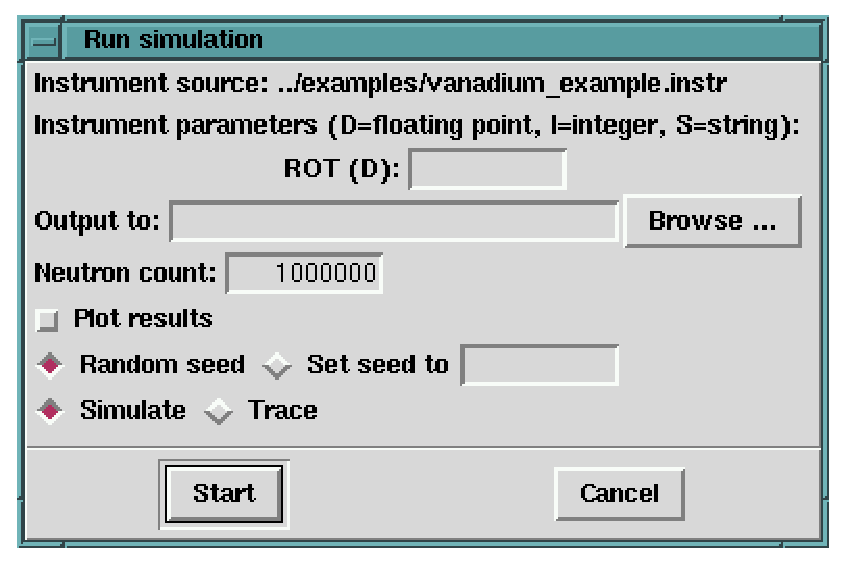
\includegraphics[width=0.45\textwidth]{figures/mcgui-run.eps}
  \end{center}
\caption{The run dialog in \texttt{mcgui}.}
\label{fig:mcgui-run}
\end{figure}
%
The run dialog is used to run simulations. It allows the entry of
instrument parameters as well as the specifications of options for
running the simulation (see section~\ref{s:run-sim} for details). It
also allows to run the \verb+mcdisplay+ (section~\ref{s:mcdisplay}) and
\verb+mcplot+ (section~\ref{s:mcplot}) front-ends together with the
simulation.

The meaning of the different fields is as follows:
\begin{description}
\item[Instrument parameters] allows the setting of the values for
  the input parameters of the instrument. The type of each instrument
  parameter is given in parenthesis after each name. Floating point
  numbers are denoted by (D) (for the C type ``\verb+double+''), (I)
  denotes integer parameters, and (S) denotes strings.
\item[Output to] allows the entry of a directory to store the
  resulting data files in (like the \verb+--dir+ option). If no name is
  given, the results are put in the current directory, to be overwritten
  by the next simulation.
\item[Neutron count] sets the number of neutron histories to
  simulate (the \verb+--ncount+ option).
\item[Plot results] -- if checked, the \verb+mcplot+ front-end will be run
  after the simulation has finished, and the plot dialog will pop up
  (see below).
\item[Random seed/Set seed to] selects between using a random seed (different
  in each simulation) for the random number generator, or using a fixed
  seed (to reproduce results for debugging).
\item[Simulate/Trace] selects between running the simulation
  normally, or using the \verb+mcdisplay+ front-end.
\item[Start] runs the simulation.
\item[Cancel] aborts the dialog.
\end{description}

Before running the simulation, the instrument definition is
automatically compiled if it is newer than the generated C file (or if the C file
is newer than the executable). The executable is
assumed to have a \verb+.out+ suffix in the filename.


\subsubsection{The plot dialog}
\begin{description}
\item[Monitors and detectors] lists all the one- and
  two-dimensional detectors in the instrument. By double-clicking, one plots
  the data in the plot window.
\item[Plot] plots the selected detector in the plot window, just
  like double-clicking its name.
\item[Overview plot] plots all the detectors together in the plot
  window.
\item[B\&W postscript] prompts for a file name and saves the
  current plot as a black and white postscript file. This can
  subsequently be printed on a postscript printer.
\item[Colour postscript] creates a colour postscript file of the
  current plot.
\item[Close] ends the dialog.
\end{description}


\subsubsection{The editor window}

The editor window provides a simple editor for creating and modifying
instrument definitions. Apart from the usual editor functions, the
``Insert'' menu provides some functions that aid in the construction of
the instrument definitions:
\begin{description}
\item[Instrument template] inserts the text for a simple instrument
  skeleton in the editor window.
\item[Component\ldots] opens up a dialog window with a list of all
  the components available for use in McStas. Selecting a component will
  display a description. Double-clicking will open up a dialog window
  allowing the entry of the values of all the parameters for the
  component (figure~\ref{f:comp_dialog}). See section~\ref{s:instrdefs}
  for details of the meaning of the different fields.

The dialog will also pick up those of the users own components that are
  present in the current directory when \verb+mcgui+ is started. See
  section~\ref{s:mcdoc} for how to write components to integrate well
  with this facility.
\item[\textit{Type}] These menu entries give quick access to the entry
  dialog for the various components available.
\end{description}
\begin{figure}[tbp]
  \begin{center}
    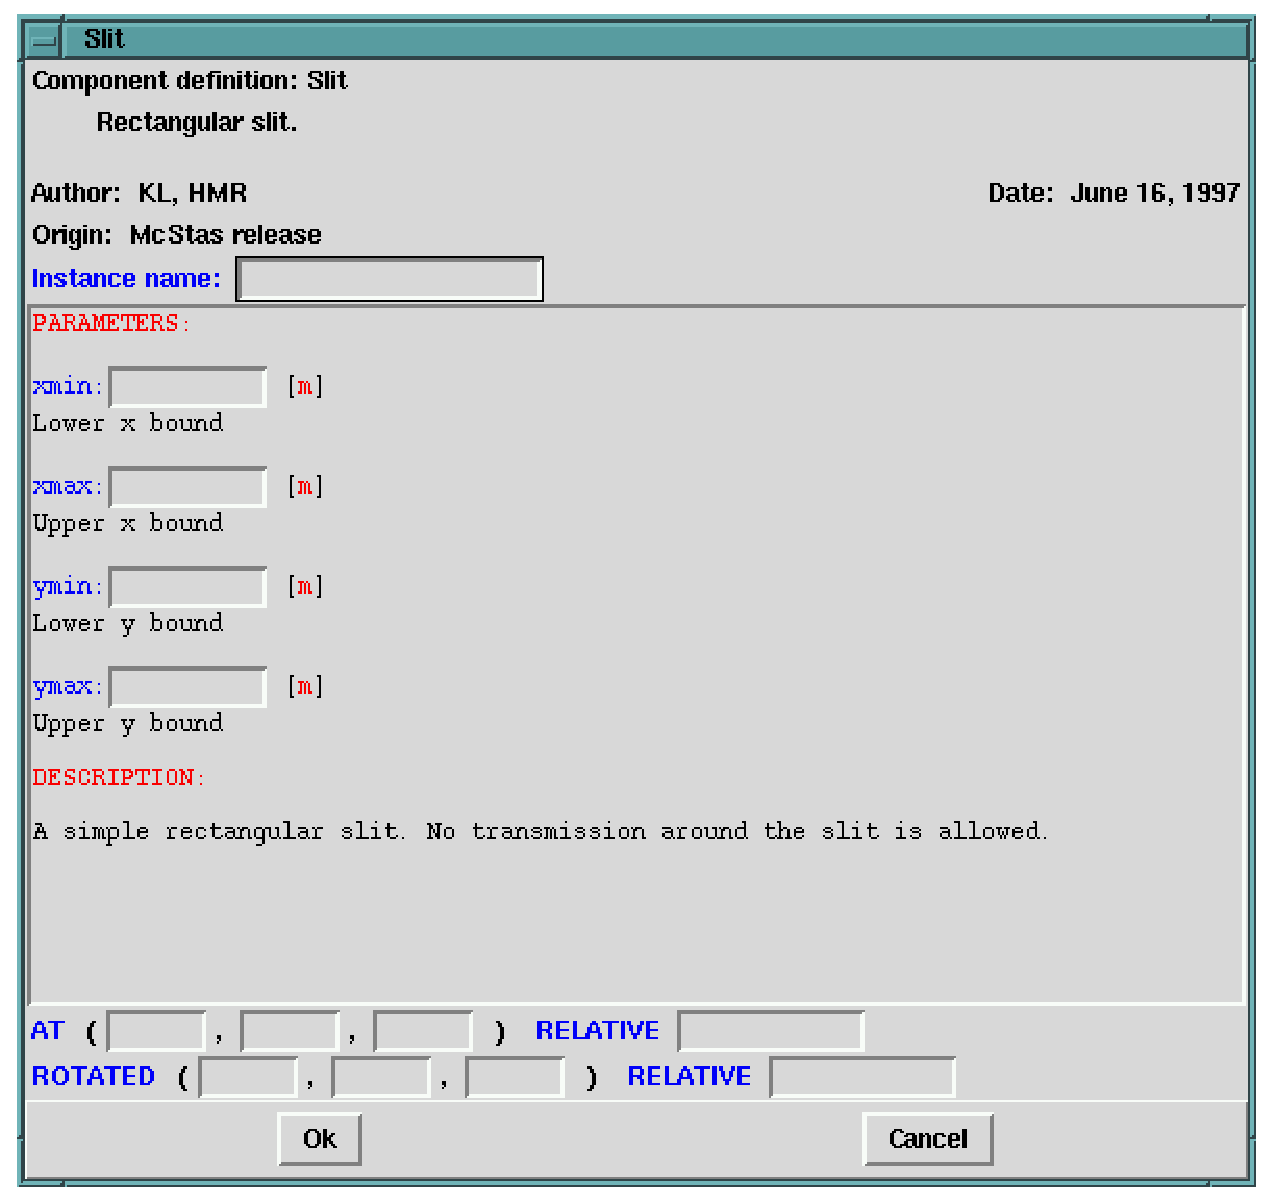
\includegraphics[width=0.55\textwidth]{figures/comp_dialog.eps}
    \caption{Component parameter entry dialog.}
    \label{f:comp_dialog}
  \end{center}
\end{figure}


To use the \verb+mcgui+ front-end, the programs Perl, Perl/Tk, PGPLOT, PgPerl,
and PDL must all be properly installed on the system. It may
be necessary to set the \verb+PGPLOT_DIR+ environment variable; consult
the documentation for PGPLOT on the local system in case of difficulty.


\subsection{Running simulations with automatic compilation}
\label{s:mcrun}

The \verb+mcrun+ front-end provides a convenient command-line
interface for running simulations with the same automatic compilation
features available in the \verb+mcgui+ front-end. It also provides a
facility for running a series of simulations while varying an input
parameter, thereby replacing the old \verb+gscan+ front-end.

The command
\begin{quote}
  \texttt{mcrun {\it sim} {\it args\/} \ldots}
\end{quote}
will compile the instrument definition \texttt{{\it sim}.instr} (if
necessary) into an executable simulation \texttt{{\it sim}.out}. It
will then run \texttt{{\it sim}.out}, passing the argument list {\it
  args}

The possible arguments are the same as those accepted by the simulations
themselves as described in section~\ref{s:run-sim}, with the following
extensions:
\begin{itemize}
\item The \verb+-c+ or \verb+--force-compile+ option may be used to for
  the recompilation of the instrument definition, regardless of file
  dates. This may be needed in case any component definitions are
  changed (in which case \verb+mcrun+ does not automatically recompile),
  or if a new version of McStas has been installed.
\item The \texttt{-p {\it file}} or \texttt{--param={\it file}} option
  may be used to specify a file containing assignment of values to the
  input parameters of the instrument definition. The file should consist
  of specifications of the form \texttt{{\it name\/}={\it value\/}}
  separated by spaces or line breaks. Multiple \verb+-p+ options may be
  given together with direct parameter specifications on the command
  line. If a parameter is assigned multiple times, later assignments
  override previous ones.
\item The \texttt{-N {\it count}} or \texttt{--numpoints={\it count}} option
  may be used to perform a series of \textit{count\/} simulations while
  varying one or more parameters within specified intervals. Such a
  series of simulations is called a \emph{scan}. To specify
  an interval for a parameter \textit{X}, it should be assigned two
  values separated with a comma. For example, the command
\begin{verbatim}
    mcrun sim.instr -N4 X=2,8 Y=1
\end{verbatim}
would run the simulation defined in \verb+sim.instr+ four times, with
\textit{X} having the values 2, 4, 6, and 8, respectively.

After running the simulation, the results will be written to the file
\verb+mcstas.dat+ by default. This file contains one line for each
simulation run giving the values of the scanned input variables along
with the intensity and estimated error in all detectors. Additionally, a
file \verb+mcstas.sim+ is written that can be read by the \verb+mcplot+
front-end to plot the results on the screen or in a Postscript file, see
section~\ref{s:mcplot}.
\item When doing a scan, the \texttt{-f {\it file}} and
  \texttt{--file={\it file}} options make \verb+mcrun+ write the output
  to the files \texttt{{\it file\/}.dat} and \texttt{{\it file\/}.sim}
  instead of the default names.
\item When doing a scan, the \texttt{-d {\it dir}} and
  \texttt{--dir={\it dir}} options make \verb+mcrun+ put all output in a
  newly created directory \textit{dir}. Additionally, the directory will
  have subdirectories \verb+1+, \verb+2+, \verb+3+,\ldots containing all
  data files output from the different simulations. When the \verb+-d+
  option is not used, no data files are written from the individual
  simulations (in order to save disk space).
\end{itemize}

The \verb+mcrun+ front-end requires a working installation of Perl to run.


\subsection{The \texttt{gscan} front-end}
\label{gscan}

The front-end \verb+gscan+ is obsolete from version~1.3 of McStas, and
is included only for backwards compatibility. The front-end~\verb+mcrun+
(section~\ref{s:mcrun}) includes all the functionality of the old
\verb+gscan+ front-end and should be used instead.


\subsection{Graphical display of simulations}
\label{s:mcdisplay}

The front-end \verb+mcdisplay+ is a graphical debugging tool.
It presents a schematic drawing of the instrument
definition, showing the position of the components and the paths of the
simulated neutrons through the instrument. It is thus very useful for
debugging a simulation, for example to spot components in the wrong
position or to find out where neutrons are getting lost. The graphics
is shown on an X Windows display.

To use the \verb+mcdisplay+ front-end with a simulation, run it as
follows:
\begin{quote}
  \verb+mcdisplay sim.out +{\it args \ldots}
\end{quote}
where \verb+sim+ is the name of the simulation program generated with
\MCS\ and \textit{args \ldots} are the normal command line arguments for
the simulation, as explained above. 
This will view the instrument from above. A
multi-display that shows the instrument from three directions
simultaneously can be shown using the \verb+--multi+ option:
\begin{quote}
  \verb+mcdisplay --multi sim.out +{\it args \ldots}
\end{quote}
The \verb+mcdisplay+ front-end can also be run from the \verb+mcgui+ front-end.

Click the left mouse button in the graphics window or hit the space key
to see the display of successive neutron trajectories. The `P' key saves
a postscript file containing the current display that can be sent to the
printer to obtain a hardcopy; the `C' key produces color postscript. 
To stop the simulation
prematurely, type `Q' or use control-C as normal in the window in which
\verb+mcdisplay+ was started.

To see details in the instrument, it is possible to zoom in on a part of
the instrument using the middle mouse button (or the `Z' key on systems
with a one- or two-button mouse). The right mouse button (or the `X'
key) resets the zoom. Note that after zooming, the units on the
different axes may no longer be equal, and thus the angles as seen on
the display may not match the actual angles.

Another way to see details while maintaining an overview of the
instrument is to use the \verb+--zoom=+\textit{factor} option. This
magnifies the display of each component along the selected axis only,
{\em e.g.} a Soller collimator is magnified perpendicular to the neutron beam
but not along it. This option may produce rather strange visual effects
as the neutron passes between components with different coordinate
magnifications, but it is occasionally useful.

When debugging, it is often the case that one is interested only in
neutrons that reach a particular component in the instrument. For
example, if there is a problem with the sample one may prefer not to see
the neutrons that are absorbed in the monochromator shielding. For these
cases, the \verb+--inspect=+\textit{comp\/} option is useful. With this
option, only neutrons that reach the component named \textit{comp\/} are
shown in the graphics display.

See section~\ref{s:comp-mcdisplay} for how to make new components work
with the \verb+mcdisplay+ front-end. The \verb+mcdisplay+ front-end
requires the Perl, the PGPLOT, and the PGPerl packages to be installed.


\subsection{Plotting the results of a simulation}
\label{s:mcplot}

The front-end \verb+mcplot+ is a program that produces
plots of all the detectors in a simulation, and it is thus useful to get
a quick overview of the simulation results.

In the simplest case, the front-end is run simply by typing
\begin{verbatim}
    mcplot
\end{verbatim}
This will plot any simulation data stored in the current directory,
which is where simulations put their results by default. If the
\verb+--dir+ or \verb+--file+ options have been used (see
section~\ref{s:run-sim}), the name of the file or directory should be
passed to mcplot, {\em e.g.} ``\texttt{mcplot {\it dir}}'' or ``\texttt{mcplot
  {\it file}}''.

The initial display shows plots for each detector in the simulation.
Clicking the left mouse button on a plot produces a full-window version
of that plot. The `P' key saves a postscript file containing the current
plot that can be sent to the printer to obtain a hardcopy; the `C' key
produces color postscript. 
The `Q' key quits the program (or CTRL-C in the controlling
terminal may be used as normal).

To use the \verb+mcplot+ front-end, the programs Perl, PGPLOT, PgPerl,
and PDL must all be properly installed on the system.



\subsection{Plotting resolution functions}
\label{s:mcresplot}

The \verb+mcresplot+ front-end is used to plot the resolution function
of a triple-axis 
%or inverse geometry time-of-flight 
spectrometer, as
calculated by the Res\_sample component. 
%(see section~\ref{s:res_sample}). 
This front-end 
has been included in the release since it may be useful
despite its somewhat rough user interface.

The \verb+mcresplot+ front-end is run with the command
\begin{quote}
  \texttt{mcresplot {\it file\/}}
\end{quote}
Here, {\it file\/} is the name of a file output from a simulation using
the Res\_monitor component.
% (section~\ref{s:res_monitor}). 
The front-end
will open two windows. One shows a three-dimensional visualization of
the resolution function using the two components of $\boldsymbol{Q}$ in
the scattering plane and $\omega$. The plot may be rotated using the
mouse while pressing the left button, and zoomed while pressing the
right button.

The other window displays the covariance matrix of the resolution
function and the resulting resolution matrix. This is mainly useful for
triple-axis spectrometers. The four bottom plots visualize the
covariance matrix using four different projections. The top left corner
shows histograms of the resolution function along the three axes of
$\boldsymbol{Q}$ and along the $\omega$ axis.

Pressing the ``Q'' key while the three-dimensional window is active
switches to a combined plot where the yellow dots show the resolution
function and the red dots show the covariance matrix. A second press of
the ``Q'' key ends the front-end program.

To use the \verb+mcresplot+ front-end, the programs Perl, PGPLOT, PgPerl,
and PDL must all be properly installed on the system.



\section{Analyzing and visualizing the simulation results}
\label{s:analyze}

To analyze simulation results, one uses the same tools as for analyzing
experimental data, \textit{i.e}. programs such as the MATLAB packages
Mview and Mfit %\cite{mfit} 
used at Ris\o. The output files from
simulations are simply columns of ASCII text that most programs should
be able to read. A future version of \MCS\ will support output in the
NeXus format~\cite{nexus_webpage}.

One-dimensional histogram detectors (time-of-flight, energy-sensitive)
write one line for each histogram bin. Each line contains a number
identifying the bin (\textit{i.e}.\ the time-of-flight) followed by
three numbers: the simulated intensity, an estimate of the statistical
error as explained in section~\ref{s:staterror}, and the number of
neutron events for this bin.

Two-dimensional histogram detectors (position sensitive detectors)
output $M$ lines of $N$ numbers representing neutron intensities, where
$M$ and $N$ are the number of bins in the two dimensions. The
two-dimentional detectors do not store any error estimates since this is
seldom useful, however if needed it can be obtained using
\verb+MC_GETPAR+ in the \verb+FINALLY+ section of the instrument
definition, see section~\ref{s:comp-declare}.

Single-point detectors output the neutron intensity, the estimated
error, and the neutron event count as numbers on the
terminal. (The results from a series of simulations may be combined in a
data file using the \verb+mcrun+ front-end as explained in
section~\ref{s:mcrun}).

Both one- and two-dimentional detector output by default start with a
header of comment lines, all beginning with the `\verb+#+' character.
This header gives such information as the name of the instrument used in
the simulation, the values of any instrument parameters, the name of the
detector component for this data file, \textit{etc}. The headers may be
disabled using the \verb+--ascii-only+ option in case the file must be
read by a program that cannot handle the headers.

In addition to the files written for each one- and two-dimensional
detector component, another file (by default named \verb+mcstas.sim+) is
also created. This file is in a special \MCS\ ASCII format. It contains
all available information about the instrument definition used for the
simulation, the parameters and options used to run the simulation, and
the detector components present in the instrument. It is read by the
\verb+mcplot+ front-end (see section~\ref{s:mcplot}). This file stores
the results from single detectors, but by default contains only pointers
(in the form of file names) to data for one- and two-dimensional
detectors. By storing data in separate files, reading the data with
programs that do not know the special \MCS\ file format is
simplified. The \verb+--file+ option may be used to store all data
inside the \verb+mcstas.sim+ file instead of in separate files.

Note that the neutron event counts in detectors is typically not very
meaningful except as a way to measure the performance of the
simulation. Use the simulated intensity instead whenever analysing
simulation data.
